\documentclass[11pt,a4paper]{article}

\usepackage{kotex}
\usepackage{amsmath,amssymb,amsthm,mathtools,bm}
\usepackage{booktabs,tabularx,longtable,array}
\usepackage{graphicx}
\usepackage{caption}
\usepackage{subcaption}
\usepackage{geometry}
\usepackage{enumitem}
\usepackage{xcolor}
\usepackage{hyperref}
\usepackage{listings}
\usepackage{float}
\usepackage{tcolorbox}
\tcbuselibrary{breakable,skins}

\geometry{margin=25mm}
\graphicspath{{report_figures/}}
\hypersetup{
  colorlinks=true,
  linkcolor=blue!60!black,
  citecolor=blue!60!black,
  urlcolor=blue!60!black
}
\setlist[itemize]{leftmargin=2em}
\setlist[enumerate]{leftmargin=2em}
\lstset{
  basicstyle=\ttfamily\small,
  breaklines=true,
  frame=single,
  columns=fullflexible
}
\sloppy

% ---- 수학 매크로 ----
\newcommand{\E}{\mathcal{E}}
\newcommand{\N}{\mathcal{N}}
\newcommand{\Hcal}{\mathcal{H}}
\newcommand{\Tr}{\operatorname{Tr}}
\newcommand{\Choi}{C_{\mathcal{E}}}
\newcommand{\id}{\mathrm{id}}
\newcommand{\Pos}{\mathrm{Pos}}
\newcommand{\Dens}{\mathrm{D}}
\newcommand{\Lin}{\mathrm{L}}
\newcommand{\diamondnorm}[1]{\left\lVert #1 \right\rVert_{\diamond}}
\newcommand{\onenorm}[1]{\left\lVert #1 \right\rVert_{1}}
\newcommand{\rank}{\operatorname{rank}}
\newcommand{\vecop}{\operatorname{vec}}
\DeclareMathOperator{\sgn}{sgn}

% ---- 정리 환경 ----
\theoremstyle{definition}
\newtheorem{definition}{정의}[section]
\newtheorem{example}{예}[section]
\theoremstyle{plain}
\newtheorem{theorem}{정리}[section]
\newtheorem{proposition}{명제}[section]
\newtheorem{property}{성질}[section]
\newtheorem{corollary}{따름정리}[section]
\theoremstyle{remark}
\newtheorem*{remark}{참고}

% ---- 색상 상자 ----
\newtcolorbox{conceptbox}[1]{
  colback=blue!4!white, colframe=blue!50!black,
  fonttitle=\bfseries, title={#1},
  breakable, boxrule=0.6pt, arc=2pt}
\newtcolorbox{intuitionbox}{
  colback=green!4!white, colframe=green!45!black,
  breakable, boxrule=0.6pt, arc=2pt,
  left=4pt,right=4pt,top=3pt,bottom=3pt}
\newtcolorbox{mathbox}[1]{
  colback=orange!4!white, colframe=orange!55!black,
  fonttitle=\bfseries, title={#1},
  breakable, boxrule=0.6pt, arc=2pt}

\title{\textbf{양자 채널의 Choi 표현을 이용한 채널 분석과 응용\\[4pt]
\large{--- 수식으로 보는 이론 해설본 ---}}}
\author{Choi Representation Multi-Agent Project}
\date{\today}

\begin{document}
\maketitle

\begin{abstract}
이 문서는 같은 프로젝트의 ``초심자용 안내서''를 \textbf{이론적으로 보강한 해설본}이다. 안내서가 각 개념을 주로 말로 설명했다면, 이 해설본은 같은 개념들을 \emph{정의(definition)}, 그것이 만족하는 \emph{성질(property)}, 그리고 핵심 \emph{정리(theorem)}의 형태로 수식을 갖추어 다시 쓴다. 목표는 ``Choi 행렬을 쓰면 채널의 물리성·성능·시간 상관·구별 가능성이 모두 선형대수 조건으로 환원된다''는 주장을, 단순한 직관이 아니라 \emph{검증 가능한 등식과 부등식}으로 뒷받침하는 것이다.

본문의 핵심 골격은 다음과 같다. 밀도행렬·텐서곱·부분 대각합을 엄밀히 정의한 뒤(2장), 양자 채널의 세 가지 동치 표현(Kraus, Stinespring, Choi)과 그 사이를 잇는 \textbf{Choi--Jamio{\l}kowski 동형사상}을 정리로 제시한다(3장). 이어서 채널의 완전양성성(CP)이 Choi 행렬의 양의 준정부호성과 동치이고($\E \text{ CP}\iff C_\E\succeq0$), 대각합 보존(TP)이 부분 대각합 조건과 동치임($\E\text{ TP}\iff\Tr_B C_\E=I_A$)을 증명 개요와 함께 다룬다. 그 위에서 다섯 가지 작업---표현 변환 검증, process tomography, diamond norm 기반 channel discrimination, quantum comb를 이용한 non-Markovian 분석, 시각화---을 각각 fidelity, diamond norm, Helstrom 한계, BLP/RHP measure, link product 같은 \emph{정량적 도구의 정의}와 함께 전개한다. 모든 그림·표·수치 결과는 안내서 및 원본 보고서와 동일하게 유지하되, 각 수치가 \emph{어떤 식으로부터 나오는지}를 명시한다(예: $F_{\mathrm{avg}}=\frac{dF_{\mathrm{pro}}+1}{d+1}$로 표의 값들이 재현됨을 확인).
\end{abstract}

\tableofcontents
\newpage

%==================================================================
\section{이 해설본을 읽는 방법}
%==================================================================

이 문서는 ``초심자용 안내서''와 짝을 이룬다. 따라서 다음과 같이 읽기를 권한다.

\begin{itemize}
  \item 개념의 \emph{의미}와 \emph{직관}이 궁금하면 먼저 안내서(\texttt{FINAL\_REPORT\_ko\_beginner.pdf})를 보는 것이 빠르다.
  \item 그 개념이 \emph{정확히 어떤 수학적 대상}이고 \emph{어떤 등식/부등식을 만족하는지}를 확인하려면 이 해설본을 본다.
\end{itemize}

본문에는 세 종류의 상자가 있다. 파란 \textbf{개념 상자}는 용어를 도입하고, 초록 \textbf{직관 요약}은 한 문장 요약을 주며, 새로 추가된 주황 \textbf{수식 상자}는 그 개념의 정의식과 핵심 성질을 모아 둔다. 또한 \emph{정의 / 성질 / 명제 / 정리}는 번호가 붙은 정리 환경으로 제시하여, 어디서 무엇이 ``증명되었는지''를 추적할 수 있게 했다.

\begin{conceptbox}{표기 약속(notation)}
\begin{itemize}[leftmargin=1.4em]
  \item $\Hcal_A,\Hcal_B$: 유한 차원 복소 Hilbert 공간, $d_A=\dim\Hcal_A$ 등. 큐비트는 $d=2$.
  \item $\Lin(\Hcal)$: $\Hcal$ 위 선형연산자 전체. $\Pos(\Hcal)=\{X\succeq0\}$, $\Dens(\Hcal)=\{\rho\succeq0,\ \Tr\rho=1\}$(밀도행렬 집합).
  \item $X^\dagger$: 켤레전치(에르미트 수반), $X^T$: 전치, $\overline{X}$: 성분별 켤레복소.
  \item $\succeq0$: 양의 준정부호(positive semidefinite, 모든 고유값 $\ge0$).
  \item $\onenorm{X}=\Tr\sqrt{X^\dagger X}$: 대각합 노름(trace norm, 특이값의 합).
  \item $I_A$: $\Hcal_A$ 위 항등연산자. $\{|i\rangle\}$: 계산기저(computational basis).
  \item 파울리 행렬 $X,Y,Z$와 $\vec\sigma=(X,Y,Z)$.
\end{itemize}
\end{conceptbox}

%==================================================================
\section{준비 1 --- 상태, 텐서곱, 부분 대각합의 수식}
%==================================================================

\subsection{밀도행렬: 정의와 성질}

\begin{definition}[밀도행렬]
계 $\Hcal$의 상태는 다음을 만족하는 연산자 $\rho\in\Lin(\Hcal)$이다.
\[
\rho=\rho^\dagger,\qquad \rho\succeq0,\qquad \Tr\rho=1 .
\]
순수 상태 $|\psi\rangle$에 대해서는 $\rho=|\psi\rangle\langle\psi|$, 일반적으로는 확률분포 $\{p_k\}$와 상태 $\{|\psi_k\rangle\}$에 대해 $\rho=\sum_k p_k|\psi_k\rangle\langle\psi_k|$.
\end{definition}

\begin{property}[밀도행렬의 기본 성질]\label{prop:density}
임의의 밀도행렬 $\rho$에 대하여 다음이 성립한다.
\begin{enumerate}[label=\textup{(\roman*)}]
  \item \textbf{스펙트럼 분해:} $\rho=\sum_i \lambda_i|e_i\rangle\langle e_i|$, $\lambda_i\ge0$, $\sum_i\lambda_i=1$. 즉 고유값들이 하나의 확률분포를 이룬다.
  \item \textbf{기댓값:} 관측량 $A=A^\dagger$에 대해 $\langle A\rangle=\Tr(\rho A)$.
  \item \textbf{순도(purity):} $\Tr(\rho^2)=\sum_i\lambda_i^2\le1$이고, 등호는 $\rho$가 순수 상태일 때 그리고 그때만 성립한다.
\end{enumerate}
\end{property}

\begin{proof}[증명 개요]
(i)~$\rho$가 에르미트이고 $\succeq0$이므로 스펙트럼 정리로 실수 고유값 $\lambda_i\ge0$을 가지며, $\Tr\rho=\sum_i\lambda_i=1$. (ii)~선형성과 $\Tr$의 순환성으로 즉시 성립. (iii)~$\sum_i\lambda_i=1,\ \lambda_i\ge0$이면 $\sum\lambda_i^2\le(\sum\lambda_i)^2=1$이고, 등호는 한 $\lambda$만 $1$일 때, 즉 rank-1(순수)일 때 성립.
\end{proof}

성질 \ref{prop:density}의 ``고유값이 음이 아니다''와 정의의 ``$\Tr\rho=1$''이라는 두 조건은 이후 채널의 CP/TP 조건으로 \emph{그대로 일반화}된다. 이것이 이 보고서 전체를 관통하는 한 줄기다.

\subsection{대각합과 부분 대각합}

\begin{definition}[부분 대각합]
$\Hcal_A\otimes\Hcal_B$ 위 연산자 $M$에 대해, $B$에 대한 부분 대각합 $\Tr_B:\Lin(\Hcal_A\otimes\Hcal_B)\to\Lin(\Hcal_A)$은
\[
\Tr_B(M)=\sum_{k}(I_A\otimes\langle k|_B)\,M\,(I_A\otimes|k\rangle_B)
\]
로 정의된다. 여기서 $\{|k\rangle_B\}$는 $\Hcal_B$의 임의의 정규직교기저이며, 정의는 기저 선택에 무관하다.
\end{definition}

\begin{property}[부분 대각합의 성질]
$\Tr_B$는 선형이고, $\Tr_A\circ\Tr_B=\Tr$이며, 곱 상태에 대해 $\Tr_B(\rho_A\otimes\rho_B)=\rho_A\,\Tr(\rho_B)$이다. 또한 $M\succeq0$이면 $\Tr_B(M)\succeq0$이다(부분 대각합은 양성을 보존한다). 합동 상태 $\rho_{AB}$의 환원 상태는 $\rho_A=\Tr_B(\rho_{AB})$로 주어진다.
\end{property}

\begin{intuitionbox}
\textbf{직관:} 부분 대각합은 ``한쪽 계를 측정하지 않고 무시했을 때 남는 상태''를 주는 \emph{유일한 물리적 사상}이다. 뒤에서 TP 조건이 ``출력 쪽 부분 대각합''으로, 채널 작용이 ``입력 쪽 부분 대각합''으로 표현된다.
\end{intuitionbox}

\subsection{텐서곱과 최대 얽힘 상태}

\begin{definition}[최대 얽힘 상태]
$\Hcal_A\cong\Hcal_B\cong\mathbb{C}^d$일 때 (비정규화) 최대 얽힘 벡터를
\[
|\Omega\rangle=\sum_{i=1}^{d}|i\rangle_A\otimes|i\rangle_B,\qquad \langle\Omega|\Omega\rangle=d,
\]
정규화 버전을 $|\Phi\rangle=\tfrac{1}{\sqrt d}|\Omega\rangle$로 둔다. 큐비트($d=2$)에서는 $|\Phi\rangle=\tfrac1{\sqrt2}(|00\rangle+|11\rangle)$.
\end{definition}

\begin{property}[ricochet/전치 항등식]\label{prop:ricochet}
임의의 연산자 $M$에 대하여
\[
(M\otimes I)\,|\Omega\rangle=(I\otimes M^{T})\,|\Omega\rangle .
\]
\end{property}
\begin{proof}
$(M\otimes I)|\Omega\rangle=\sum_i (M|i\rangle)\otimes|i\rangle=\sum_{i,j}M_{ji}|j\rangle\otimes|i\rangle$. 한편 $(I\otimes M^T)|\Omega\rangle=\sum_i|i\rangle\otimes(M^T|i\rangle)=\sum_{i,j}(M^T)_{ji}|i\rangle\otimes|j\rangle=\sum_{i,j}M_{ij}|i\rangle\otimes|j\rangle$. 둘째 식에서 $i\leftrightarrow j$로 더미 지표를 바꾸면 첫째 식과 같다.
\end{proof}

성질 \ref{prop:ricochet}은 Choi 행렬에서 채널 작용을 복원하는 공식(정리 \ref{thm:recover})과, ``채널을 한쪽에만 걸어도 다른 쪽 상관에 흔적이 남는다''는 SDP 절의 핵심을 수식으로 떠받친다.

%==================================================================
\section{준비 2 --- 양자 채널과 세 가지 동치 표현}
%==================================================================

\subsection{양자 채널: 정의와 CP/TP}

\begin{definition}[양자 채널]
선형사상 $\E:\Lin(\Hcal_A)\to\Lin(\Hcal_B)$가 다음을 만족하면 양자 채널(CPTP 사상)이라 한다.
\begin{itemize}[leftmargin=1.6em]
  \item \textbf{대각합 보존(TP):} 모든 $X$에 대해 $\Tr[\E(X)]=\Tr[X]$.
  \item \textbf{완전양성성(CP):} 모든 $n\ge1$에 대해 확장된 사상 $\E\otimes\id_n:\Lin(\Hcal_A\otimes\mathbb C^n)\to\Lin(\Hcal_B\otimes\mathbb C^n)$이 양성을 보존한다. 즉 $X\succeq0\Rightarrow(\E\otimes\id_n)(X)\succeq0$.
\end{itemize}
\end{definition}

\begin{mathbox}{왜 ``양성''이 아니라 ``완전양성''인가}
양성($n=1$)만 요구하면 부족하다. 고전적 반례는 전치 사상 $T(\rho)=\rho^T$로, $T$는 양성이지만 완전양성이 아니다. 실제로 큐비트 한 쌍의 최대 얽힘 상태 $|\Phi\rangle\langle\Phi|$에 $T\otimes\id$를 걸면
\[
(T\otimes\id)(|\Phi\rangle\langle\Phi|)=\tfrac12\,\mathrm{SWAP}
\]
가 되어 고유값 $-\tfrac12$를 가진다(음수!). 즉 ``남몰래 얽혀 있는 참조계''까지 고려하면 $T$는 물리적 채널이 아니다. CP는 바로 이 ``임의의 참조계 확장에서도 정당함''을 요구한다.
\end{mathbox}

\subsection{Kraus 표현과 Stinespring 표현}

\begin{theorem}[Kraus 표현]\label{thm:kraus}
$\E$가 CP일 필요충분조건은 연산자 집합 $\{K_k:\Hcal_A\to\Hcal_B\}$가 존재하여
\[
\E(\rho)=\sum_k K_k\,\rho\,K_k^\dagger
\]
로 쓰이는 것이다. 나아가 $\E$가 TP일 필요충분조건은
\[
\sum_k K_k^\dagger K_k=I_A .
\]
필요한 Kraus 연산자의 최소 개수를 \textbf{Kraus rank}라 한다.
\end{theorem}

\begin{theorem}[Stinespring 표현]\label{thm:stinespring}
$\E$가 CPTP일 필요충분조건은 보조계 $\Hcal_E$와 등거리사상(isometry) $V:\Hcal_A\to\Hcal_B\otimes\Hcal_E$($V^\dagger V=I_A$)가 존재하여
\[
\E(\rho)=\Tr_E\!\big(V\rho V^\dagger\big)
\]
로 쓰이는 것이다. $\dim\Hcal_E$는 Kraus rank만큼이면 충분하며, $V=\sum_k K_k\otimes|k\rangle_E$로 두면 정리 \ref{thm:kraus}와 일치한다.
\end{theorem}

\begin{intuitionbox}
\textbf{직관:} Kraus는 ``잡음이 여러 갈래로 일어난다'', Stinespring은 ``그 잡음은 사실 더 큰 닫힌 계의 깔끔한 unitary를 일부만 본 것''이라는 같은 사실의 두 얼굴이다. 정리 \ref{thm:kraus},~\ref{thm:stinespring},~그리고 다음의 Choi 표현은 \emph{서로 동치}다.
\end{intuitionbox}

\subsection{Choi 표현과 Choi--Jamio{\l}kowski 동형사상}

\begin{definition}[Choi 행렬, input-first 규약]
채널 $\E:\Lin(\Hcal_A)\to\Lin(\Hcal_B)$의 Choi 행렬은
\[
C_\E=\sum_{i,j}|i\rangle\langle j|_A\otimes\E(|i\rangle\langle j|)_B
     =(\id_A\otimes\E)\big(|\Omega\rangle\langle\Omega|\big)\ \in\ \Lin(\Hcal_A\otimes\Hcal_B).
\]
\end{definition}

\begin{theorem}[채널 작용의 복원]\label{thm:recover}
Choi 행렬로부터 채널 작용은
\[
\E(\rho)=\Tr_A\!\big[(\rho^{T}\otimes I_B)\,C_\E\big]
\]
로 복원된다.
\end{theorem}
\begin{proof}
$\Tr_A[(\rho^T\otimes I)C_\E]=\sum_{ij}\Tr[\rho^T|i\rangle\langle j|]\,\E(|i\rangle\langle j|)=\sum_{ij}\langle j|\rho^T|i\rangle\,\E(|i\rangle\langle j|)=\sum_{ij}\rho_{ij}\,\E(|i\rangle\langle j|)=\E(\rho)$. 여기서 $\langle j|\rho^T|i\rangle=(\rho^T)_{ji}=\rho_{ij}$를 썼다.
\end{proof}

\begin{theorem}[Choi--Jamio{\l}kowski; CP/TP의 행렬 판정]\label{thm:cj}
대응 $\E\mapsto C_\E$는 선형사상과 $\Lin(\Hcal_A\otimes\Hcal_B)$의 연산자 사이의 선형동형이며, 다음이 성립한다.
\[
\boxed{\ \E\text{ 가 CP}\iff C_\E\succeq0,\qquad
       \E\text{ 가 TP}\iff \Tr_B(C_\E)=I_A.\ }
\]
또한 $\rank(C_\E)=$ Kraus rank이고, $C_\E$의 스펙트럼 분해 $C_\E=\sum_k\mu_k|v_k\rangle\langle v_k|$로부터 Kraus 연산자가 $K_k=\sqrt{\mu_k}\,\mathrm{mat}(|v_k\rangle)$로 직접 얻어진다.
\end{theorem}

\begin{proof}[증명 개요]
($\Leftarrow$, CP)~$C_\E\succeq0$이면 $C_\E=\sum_k|w_k\rangle\langle w_k|$로 쓰고 $|w_k\rangle$를 행렬 $K_k$로 재배열($\mathrm{mat}$)하면 정리 \ref{thm:recover}에 의해 $\E(\rho)=\sum_k K_k\rho K_k^\dagger$이 되어 CP(정리 \ref{thm:kraus}). ($\Rightarrow$)~$\E$가 CP면 $C_\E=(\id\otimes\E)(|\Omega\rangle\langle\Omega|)$는 PSD 입력의 상이므로 $\succeq0$. TP 동치는
\[
\Tr_B(C_\E)=\sum_{ij}|i\rangle\langle j|\,\Tr[\E(|i\rangle\langle j|)]
=\sum_{ij}|i\rangle\langle j|\,\Tr[|i\rangle\langle j|]
=\sum_i|i\rangle\langle i|=I_A
\]
에서 마지막 등식이 모든 $i,j$에 대해 $\Tr[\E(|i\rangle\langle j|)]=\delta_{ij}$, 즉 TP와 동치이기 때문이다.
\end{proof}

\begin{mathbox}{이 한 장의 결론}
``채널이 물리적인가''라는 추상적 질문이 단 두 개의 \emph{선형대수} 점검으로 환원된다.
\[
\underbrace{C_\E\succeq0}_{\text{고유값}\,\ge0\ (\text{CP})}
\qquad\text{그리고}\qquad
\underbrace{\Tr_B(C_\E)=I_A}_{\text{부분 대각합}\,=\,\text{항등}\ (\text{TP})}.
\]
나머지 모든 장은 이 두 조건을 ``계산''하거나, 두 Choi 행렬을 ``비교''하거나, 여러 시점으로 ``확장''하는 이야기다.
\end{mathbox}

\subsection{Natural(Liouville) 표현과 표현 변환}

\begin{definition}[벡터화와 natural 표현]
열-쌓기(column-stacking) 벡터화 $\vecop(|i\rangle\langle j|)=|j\rangle\otimes|i\rangle$를 쓰면, 임의의 $A,B$에 대해 $\vecop(A\rho B)=(B^T\otimes A)\vecop(\rho)$가 성립한다. 따라서 채널 $\E(\rho)=\sum_k K_k\rho K_k^\dagger$의 natural(Liouville) 행렬은
\[
N_\E=\sum_k \overline{K_k}\otimes K_k,\qquad \vecop(\E(\rho))=N_\E\,\vecop(\rho).
\]
\end{definition}

\begin{property}[합성은 행렬곱]\label{prop:compose}
채널 합성에 대해 $N_{\E_2\circ\E_1}=N_{\E_2}N_{\E_1}$. 즉 natural 표현에서 채널을 잇는 것은 단순한 행렬 곱셈이다.
\end{property}

이상으로 한 채널에 대한 네 표현 Kraus, Stinespring, Choi, natural과 그 변환식이 모두 갖추어졌다. 4장은 이 변환들이 수치적으로 정확히 일치함을 확인한다. \emph{성질 \ref{prop:compose}}는 4장의 ``composition check''(표 \ref{tab:theory-results})를 정당화하는 식이다.

%==================================================================
\section{작업 1 --- 표현 변환의 수치 검증과 대표 채널의 닫힌 형}
%==================================================================

\subsection{대표 큐비트 채널의 명시적 표현}

먼저 이후 모든 장에서 재등장하는 세 채널을 닫힌 형(closed form)으로 적는다. Bloch 매개변수화 $\rho=\tfrac12(I+\vec r\cdot\vec\sigma)$ 아래에서 모든 큐비트 채널은 아핀사상 $\vec r\mapsto M\vec r+\vec t$로 표현된다($M\in\mathbb R^{3\times3}$, $\vec t\in\mathbb R^3$; $M$은 Pauli transfer matrix의 공간 부분).

\begin{mathbox}{depolarizing channel}
\[
\E_p(\rho)=(1-p)\rho+p\,\Tr(\rho)\tfrac{I}{2},\qquad
M=(1-p)I_3,\quad \vec t=0\ (\text{unital}).
\]
Kraus: $\{\sqrt{1-\tfrac{3p}{4}}\,I,\ \sqrt{\tfrac p4}X,\ \sqrt{\tfrac p4}Y,\ \sqrt{\tfrac p4}Z\}$. (비정규화, input-first) Choi 행렬의 고유값은
\[
\big\{\,2(1-p)+\tfrac p2\ (\times1),\quad \tfrac p2\ (\times3)\,\big\}.
\]
따라서 최소 고유값은 $\tfrac p2$이고, $p=0.3$이면 $\boxed{0.15}$ --- 표 \ref{tab:theory-results}의 값과 정확히 일치한다.
\end{mathbox}

\begin{mathbox}{amplitude damping channel}
\[
K_0=\begin{pmatrix}1&0\\0&\sqrt{1-\gamma}\end{pmatrix},\quad
K_1=\begin{pmatrix}0&\sqrt{\gamma}\\0&0\end{pmatrix},\qquad
M=\mathrm{diag}\!\big(\sqrt{1-\gamma},\sqrt{1-\gamma},\,1-\gamma\big),\ \ \vec t=(0,0,\gamma).
\]
TP 확인: $K_0^\dagger K_0+K_1^\dagger K_1=\mathrm{diag}(1,1-\gamma)+\mathrm{diag}(0,\gamma)=I$. \,
Unital 확인: $\E(I)=K_0K_0^\dagger+K_1K_1^\dagger=\mathrm{diag}(1+\gamma,1-\gamma)\neq I$이므로 \emph{unital 아님}($\vec t\neq0$). Kraus rank $=2$이므로 $\rank(C_\E)=2$ --- 표 \ref{tab:theory-results}의 $\gamma=0.3$ 행과 일치.
\end{mathbox}

\begin{mathbox}{identity channel}
$\E=\id$이면 $M=I_3,\ \vec t=0$, Kraus rank $=1$, 그리고 $C_{\id}=|\Omega\rangle\langle\Omega|$로 rank-1. ``잡음 갈래 없음''이 $\rank(C)=1$로 나타난다.
\end{mathbox}

이 세 상자가 4.2절 그림 \ref{fig:theory-choi-examples}에서 ``눈으로 본'' 패턴 차이의 수식적 근거다. identity는 rank-1(한 점에 집중), depolarizing은 대각으로 균일($\vec t=0$), amplitude damping은 중심 이동($\vec t=(0,0,\gamma)$).

\subsection{대표 채널들의 Choi 행렬(그림)}

\begin{figure}[H]
\centering
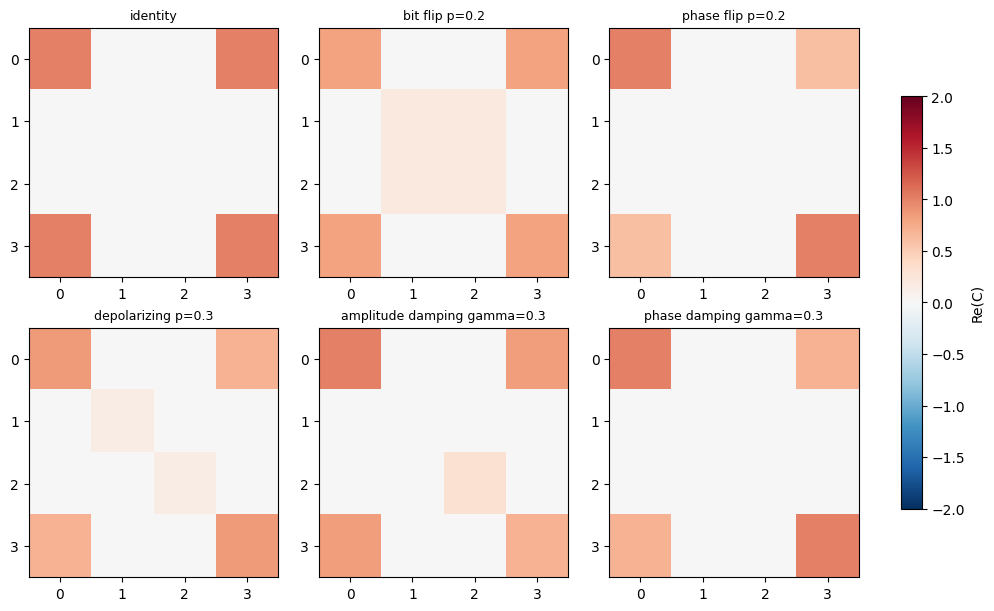
\includegraphics[width=0.94\textwidth]{fig_01_theory_01_cell6.png}
\caption{대표적인 qubit channel들의 Choi 행렬 실수부 비교. Identity는 rank-1 구조, depolarizing은 대각이 균일해지고, amplitude damping은 비대칭적 relaxation 구조를 보인다. 4.1절의 닫힌 형($\vec t,\,M,\,$고유값)이 이 패턴을 정량적으로 설명한다.}
\label{fig:theory-choi-examples}
\end{figure}

\begin{property}[TP와 unitality는 다른 조건]
$\E$가 TP $\iff\Tr_B(C_\E)=I_A$(출력 확률 보존)인 반면, $\E$가 unital $\iff\E(I)=I\iff\Tr_A(C_\E)=I_B$(입력 측 부분 대각합). amplitude damping은 전자는 만족하나 후자는 위반한다: Bloch 그림에서 ``중심이 이동''($\vec t\neq0$)하는 것이 곧 비-unital성이다.
\end{property}

\subsection{수치 검증: ``오차 $10^{-16}$''의 의미}

\begin{mathbox}{기계 정밀도(machine precision)}
배정밀도 부동소수점의 단위 반올림은 $\varepsilon_{\mathrm{mach}}=2^{-52}\approx2.22\times10^{-16}$이다. 두 계산 결과의 차이가 $\mathcal O(\varepsilon_{\mathrm{mach}})$ 규모이면 ``수치적으로 동일''로 본다. 반대로 $\sim10^{-1}$ 규모의 차이는 진짜 차이다(예: 5.4절의 $-0.27$).
\end{mathbox}

\begin{table}[H]
\centering\small
\begin{tabularx}{\textwidth}{p{0.25\textwidth}p{0.31\textwidth}X}
\toprule
항목 & 관측값 & 해석(근거 식) \\
\midrule
Identity channel & Choi rank $=1$ & $\rank(C_\E)=$ Kraus rank(정리 \ref{thm:cj}); 잡음 branch 없음. \\
Depolarizing $p=0.3$ & min eig $=0.15$, TP=True, unital=True & 4.1절 식 $\min\mathrm{eig}=p/2=0.15\ge0\Rightarrow$ CP; $\vec t=0\Rightarrow$ unital. \\
Amplitude damping $\gamma=0.3$ & TP=True, unital=False, rank$=2$ & $\sum K_k^\dagger K_k=I$(TP), $\vec t=(0,0,\gamma)\neq0$(비-unital). \\
Random channel round-trip & error $\approx2.56\times10^{-16}$ & Choi$\to$Kraus$\to$작용(정리 \ref{thm:cj},\ref{thm:recover})이 $\mathcal O(\varepsilon_{\mathrm{mach}})$로 일치. \\
Composition check & error $\approx2.48\times10^{-16}$ & $N_{\E_2\circ\E_1}=N_{\E_2}N_{\E_1}$(성질 \ref{prop:compose}) 확인. \\
\bottomrule
\end{tabularx}
\caption{이론 파트의 주요 수치 검증 결과}
\label{tab:theory-results}
\end{table}

\begin{remark}
perturbed identity 예시에서 Choi 행렬이 에르미트이고 $\Tr_B\approx I$를 거의 만족해도 작은 음의 고유값 하나로 CP=False가 된다. 즉 정리 \ref{thm:cj}의 $C_\E\succeq0$ 조건은 ``거의''를 허용하지 않는다. 이것이 5장에서 raw reconstruction을 그대로 신뢰하면 안 되는 이유의 수식적 핵심이다.
\end{remark}

%==================================================================
\section{작업 2 --- Process Tomography: 재구성과 비교 지표의 수식}
%==================================================================

\subsection{Tomography의 수식 골격}

\begin{conceptbox}{개념: process tomography}
알 수 없는 채널 $\E$에 정보적으로 완전한(informationally complete) 입력 집합 $\{\rho_a\}$를 넣고 출력 $\E(\rho_a)$를 상태 단층촬영으로 추정한 뒤, 선형 관계 $\E(\rho_a)=\Tr_A[(\rho_a^T\otimes I)C_\E]$(정리 \ref{thm:recover})를 $C_\E$에 대해 역으로 푼다. 이를 \textbf{선형 역산(linear inversion)}이라 한다.
\end{conceptbox}

선형 역산은 측정 횟수가 유한해 생기는 통계적 요동(shot noise) 때문에 $C_\E\not\succeq0$인(즉 비물리적) 추정치를 줄 수 있다. 이때 가장 가까운 물리적 채널로 사영하는 단계가 필요하다.

\begin{definition}[CPTP 사영]
재구성된 (에르미트) 행렬 $\widehat C$에 대해, CPTP 사영은
\[
C^\star=\arg\min_{C}\ \onenorm{C-\widehat C}\quad\text{s.t.}\quad C\succeq0,\ \Tr_B(C)=I_A
\]
로 정의되는 볼록 최적화(SDP)다. MLE는 같은 제약 아래 우도를 최대화하는 변형이다.
\end{definition}

모의 기준 게이트 $X,H,\mathrm{CNOT}$의 회로는 그림 \ref{fig:qpt-target-circuits}이며, 잡음은 회로가 아니라 그 뒤에 붙는 Choi-레벨 채널로 적용된다.

\begin{figure}[H]
\centering
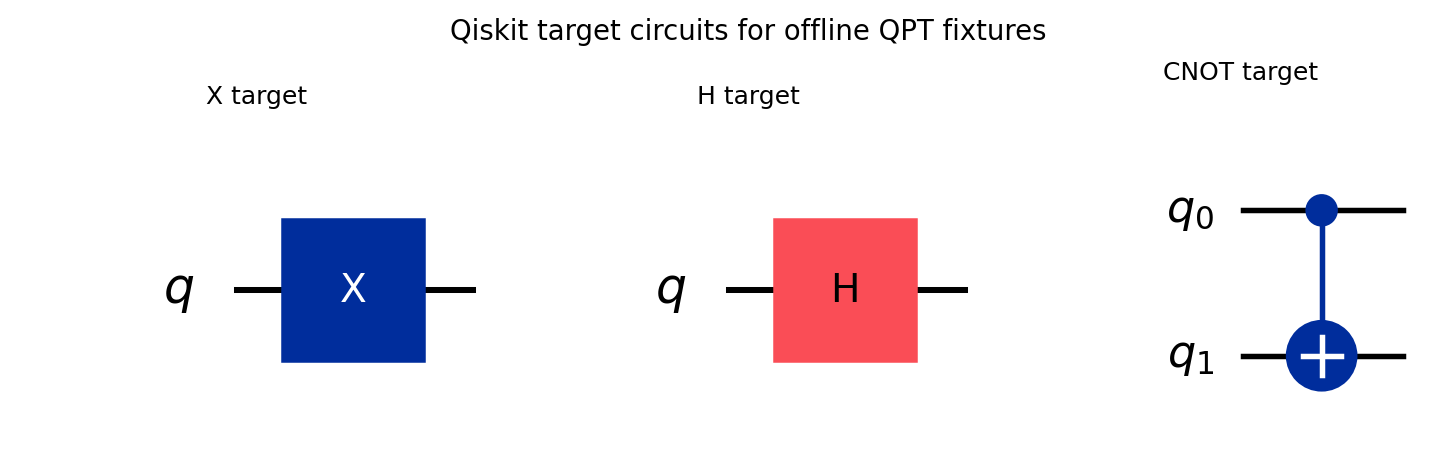
\includegraphics[width=0.92\textwidth]{fig_02_ibm_experiment_00_qiskit_circuits.png}
\caption{Offline QPT fixture의 Qiskit target circuits. $X,H$는 1큐비트, CNOT은 control $q_0$, target $q_1$의 2큐비트 게이트. Noise는 target gate 뒤의 Choi-level channel로 적용된다.}
\label{fig:qpt-target-circuits}
\end{figure}

\subsection{비교 지표: fidelity와 diamond distance의 정의}

\begin{definition}[상태 fidelity와 process fidelity]
두 상태 $\rho,\sigma$의 fidelity는 $F(\rho,\sigma)=\big(\Tr\sqrt{\sqrt\rho\,\sigma\sqrt\rho}\big)^2$. 채널 $\E$와 목표 채널 $\mathcal F$의 \textbf{process fidelity}는 정규화 Choi 상태 $\rho_\E=C_\E/d_A$로 정의한 상태 fidelity
\[
F_{\mathrm{pro}}(\E,\mathcal F)=F\!\big(\rho_\E,\rho_{\mathcal F}\big),
\]
즉 entanglement fidelity와 동치다.
\end{definition}

\begin{theorem}[average gate fidelity와의 관계]\label{thm:favg}
입력 차원 $d$에서 process(entanglement) fidelity와 average gate fidelity 사이에는
\[
\boxed{\,F_{\mathrm{avg}}=\dfrac{d\,F_{\mathrm{pro}}+1}{d+1}\,}
\]
가 성립한다(Horodecki--Nielsen 관계).
\end{theorem}

\begin{mathbox}{표 \ref{tab:qpt-results}의 수치 재현}
정리 \ref{thm:favg}로 표의 값이 그대로 나온다.
\begin{align*}
X\ (d=2):&\quad F_{\mathrm{avg}}=\tfrac{2(0.959583)+1}{3}=0.973055,\\
H\ (d=2):&\quad F_{\mathrm{avg}}=\tfrac{2(0.94)+1}{3}=0.960000,\\
\mathrm{CNOT}\ (d=4):&\quad F_{\mathrm{avg}}=\tfrac{4(0.92)+1}{5}=0.936000.
\end{align*}
즉 표의 $F_{\mathrm{pro}}$와 $F_{\mathrm{avg}}$는 독립적인 두 숫자가 아니라 한 공식으로 묶여 있다.
\end{mathbox}

\begin{definition}[diamond norm과 half-diamond distance]
Hermiticity 보존 사상 $\Delta=\E_0-\E_1$의 diamond norm은
\[
\diamondnorm{\Delta}=\max_{\rho\in\Dens(\Hcal_A\otimes\Hcal_R)}\onenorm{(\Delta\otimes\id_R)(\rho)},\qquad \dim\Hcal_R=\dim\Hcal_A,
\]
이며 최댓값은 순수 상태 $\rho=|\psi\rangle\langle\psi|$에서 달성된다. half-diamond distance는 $\tfrac12\diamondnorm{\E_0-\E_1}$.
\end{definition}

\begin{intuitionbox}
\textbf{fidelity 대 diamond:} fidelity는 Choi \emph{상태}끼리의 평균적 겹침이고, diamond는 \emph{최악의 입력}(참조계 얽힘 허용)에서의 구별 가능성이다. ``평균적으로 비슷''($F_{\mathrm{pro}}$ 큼)해도 ``최악에서는 다름''(diamond $>0$)일 수 있다 --- $X$의 $F_{\mathrm{pro}}=0.96$인데 half-diamond $=0.08\neq0$인 것이 그 예.
\end{intuitionbox}

\subsection{이상적 Choi 대 재구성된 Choi}

\begin{figure}[H]
\centering
\begin{subfigure}{0.48\textwidth}\centering
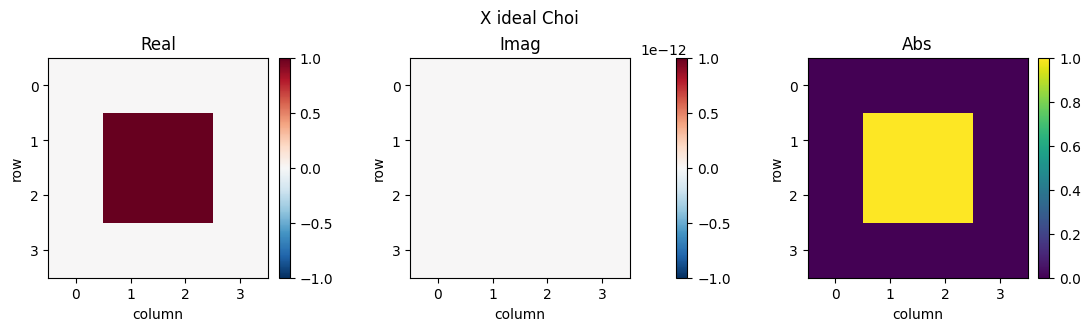
\includegraphics[width=\textwidth]{fig_02_ibm_experiment_01_cell20.png}\caption{$X$ ideal Choi}\end{subfigure}\hfill
\begin{subfigure}{0.48\textwidth}\centering
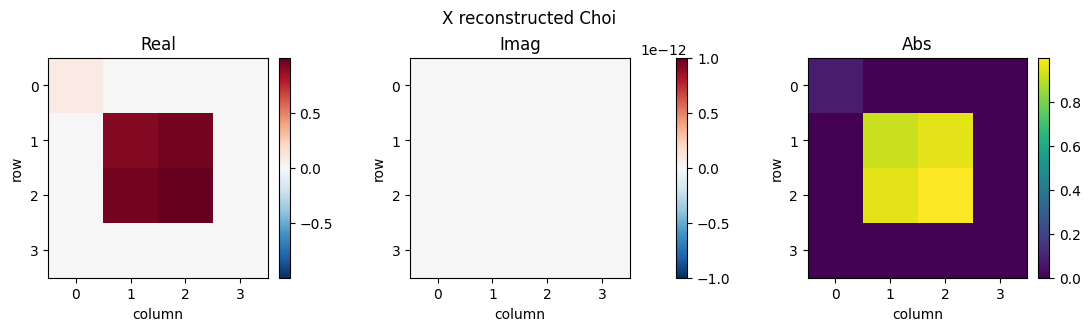
\includegraphics[width=\textwidth]{fig_02_ibm_experiment_02_cell20.png}\caption{$X$ reconstructed Choi}\end{subfigure}
\caption{$X$ gate의 ideal/reconstructed Choi 비교. 큰 구조는 유지되되 ideal pattern에서 벗어난 작은 성분이 나타난다 --- 이상적 unitary에 잡음이 더해진 형태.}
\label{fig:qpt-x-choi}
\end{figure}

그림 \ref{fig:qpt-x-choi}에서 두 행렬이 완전히 같다면 $F_{\mathrm{pro}}=1$, half-diamond $=0$이어야 한다. 실측은 $F_{\mathrm{pro}}=0.959583$, half-diamond $=0.080000$으로, 위 직관 상자의 ``평균적 유사/최악의 차이'' 구도를 정량적으로 보여준다.

\begin{figure}[H]
\centering
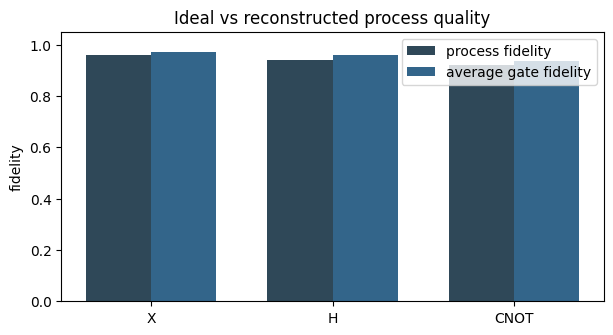
\includegraphics[width=0.74\textwidth]{fig_02_ibm_experiment_10_cell24.png}
\caption{$X,H,$ CNOT의 process/average gate fidelity. 모두 $<1$(잡음 존재). CNOT이 가장 낮다.}
\label{fig:qpt-fidelity-bars}
\end{figure}

\begin{remark}[차원이 커지면 왜 더 나빠지나]
CNOT은 2큐비트라 $C_\E\in\Lin(\mathbb C^{16})$이고, 전역 depolarizing의 Pauli error 갈래 수는 $d^2-1=15$로 1큐비트의 $3$보다 훨씬 많다. 같은 ``세기''라도 오차가 더 많은 방향으로 분산되므로 $F_{\mathrm{pro}}$가 낮아진다.
\end{remark}

\subsection{잡음의 방향성: Bloch 아핀 진단의 수식}

\begin{definition}[잔차 채널의 아핀 진단]
재구성 채널에서 이상적 게이트의 작용을 제거한 잔차를 $\vec r\mapsto M\vec r+\vec t$로 보고, 특이값 분해 $M=U\Sigma V^\dagger$, $\Sigma=\mathrm{diag}(s_1,s_2,s_3)$를 쓴다. 다음으로 분류한다.
\[
\|\vec t\|_2>\tau\ \Rightarrow\ \text{relaxation-like},
\qquad
\|\vec t\|_2\approx0\ \text{이고}\ \mathrm{spread}(s_i)\approx0\ \Rightarrow\ \text{depolarizing-like},
\]
여기서 $\mathrm{spread}(s_i)=\max_i s_i-\min_i s_i$, 임계값 $\tau=0.05$.
\end{definition}

\begin{figure}[H]
\centering
\begin{subfigure}{0.47\textwidth}\centering
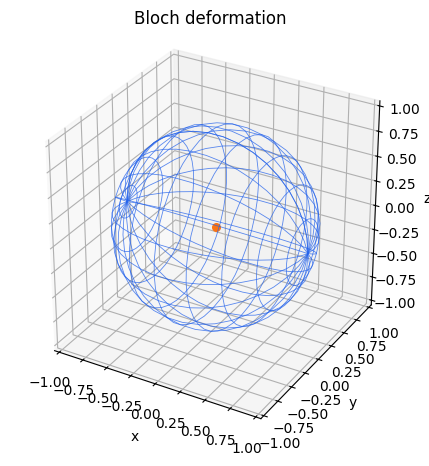
\includegraphics[width=0.82\textwidth]{fig_02_ibm_experiment_07_cell22.png}\caption{$X$ reconstructed}\end{subfigure}\hfill
\begin{subfigure}{0.47\textwidth}\centering
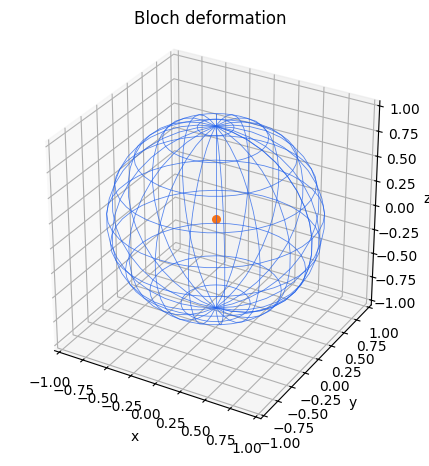
\includegraphics[width=0.82\textwidth]{fig_02_ibm_experiment_08_cell22.png}\caption{$H$ reconstructed}\end{subfigure}
\caption{재구성된 1큐비트 채널의 Bloch 변형. depolarizing-like는 균일 수축($\vec t\approx0$), amplitude-damping-like는 중심 이동($\vec t\neq0$).}
\label{fig:qpt-bloch}
\end{figure}

\begin{table}[H]
\centering\small
\begin{tabularx}{\textwidth}{lcccX}
\toprule
Gate & $\|\vec t\|_2$ & SV spread & Mean shrinkage & 진단 근거(위 정의) \\
\midrule
$X$ & 0.07999965 & 0.03916625 & 0.94611071 & $\|\vec t\|_2>0.05\Rightarrow$ relaxation-like. \\
$H$ & $1.999\times10^{-15}$ & $1.999\times10^{-12}$ & 0.92000000 & $\|\vec t\|_2,\ \mathrm{spread}\approx\mathcal O(\varepsilon)\Rightarrow$ isotropic depolarizing-like. \\
\bottomrule
\end{tabularx}
\caption{1큐비트 재구성 채널의 Bloch affine 진단 수치. $H$의 $10^{-15},10^{-12}$는 4.3절 의미에서 ``$0$''.}
\label{tab:qpt-bloch-diagnostics}
\end{table}

\begin{table}[H]
\centering\small
\begin{tabularx}{\textwidth}{lcccX}
\toprule
Gate & $F_{\mathrm{pro}}$ & $F_{\mathrm{avg}}$ & Half-diamond & 진단 \\
\midrule
$X$ & 0.959583 & 0.973055 & 0.080000 & amplitude-damping-like relaxation \\
$H$ & 0.940000 & 0.960000 & 0.060000 & depolarizing-like isotropic shrinkage \\
CNOT & 0.920000 & 0.936000 & 0.080000 & stochastic global depolarizing-like noise \\
\bottomrule
\end{tabularx}
\caption{Offline simulated QPT 결과($F_{\mathrm{avg}}$는 정리 \ref{thm:favg}로 $F_{\mathrm{pro}}$에서 유도됨).}
\label{tab:qpt-results}
\end{table}

\begin{remark}[비물리적 재구성]
선형 역산 perturbation 예시의 최소 고유값은 $-0.270000$으로, $\mathcal O(\varepsilon_{\mathrm{mach}})$가 아닌 진짜 음수다(정리 \ref{thm:cj} 위반). 따라서 CPTP 사영(5.1절 정의)으로 $\onenorm{C-\widehat C}$ 최소화 해 $C^\star\succeq0$을 회복해야 한다.
\end{remark}

%==================================================================
\section{작업 3 --- Channel Discrimination, diamond norm, SDP}
%==================================================================

\subsection{상태 구별: Holevo--Helstrom 정리}

\begin{theorem}[Holevo--Helstrom]\label{thm:helstrom}
사전확률 $\tfrac12$씩으로 두 상태 $\rho_0,\rho_1$ 중 하나가 주어질 때, 최적 구별 성공확률은
\[
p_{\mathrm{succ}}^{\max}=\frac12+\frac14\onenorm{\rho_0-\rho_1}
=\frac12+\frac12\,T(\rho_0,\rho_1),
\]
이고, 최적 측정은 $\rho_0-\rho_1$의 양/음 고유공간으로의 사영(Helstrom 측정)이다. 여기서 $T(\rho_0,\rho_1)=\tfrac12\onenorm{\rho_0-\rho_1}$는 trace distance.
\end{theorem}
\begin{proof}[증명 개요]
임의의 2-결과 POVM $\{M,I-M\}$($0\preceq M\preceq I$)에 대해 성공확률은 $\tfrac12+\tfrac12\Tr[M(\rho_0-\rho_1)]$. $\Delta=\rho_0-\rho_1=\Delta_+-\Delta_-$(양/음 부분)에 대해 $\Tr[M\Delta]\le\Tr[\Delta_+]=\tfrac12\onenorm{\Delta}$이며, $M$을 $\Delta_+$의 사영으로 두면 등호.
\end{proof}

\subsection{채널 구별: diamond norm}

채널은 입력을 고를 수 있으므로, 상태 구별을 입력에 대해 최적화한 것이 채널 구별이다. 참조계 얽힘까지 허용하면 다음이 따른다.

\begin{theorem}[채널 구별과 diamond norm]\label{thm:chandisc}
사전확률 $\tfrac12$씩으로 두 채널 $\E_0,\E_1$을 \emph{한 번} 사용해 구별하는 최적 성공확률(참조계 보조 허용)은
\[
\boxed{\,p_{\mathrm{succ}}^{\max}=\frac12+\frac14\diamondnorm{\E_0-\E_1}\,.}
\]
\end{theorem}
\begin{proof}[증명 개요]
입력 $|\psi\rangle\in\Hcal_A\otimes\Hcal_R$를 넣으면 출력은 $(\E_b\otimes\id_R)(|\psi\rangle\langle\psi|)$. 정리 \ref{thm:helstrom}을 적용하면 성공확률 $=\tfrac12+\tfrac14\onenorm{(\Delta\otimes\id_R)(|\psi\rangle\langle\psi|)}$. $|\psi\rangle$에 대해 최대화하면 정의에 의해 $\diamondnorm{\Delta}$.
\end{proof}

\begin{mathbox}{왜 참조계(ancilla)가 도움이 되는가}
diamond norm의 최댓값이 \emph{얽힌} $|\psi\rangle$에서 달성될 수 있기 때문이다. 단독(product) 입력만 쓰면 $\diamondnorm{\cdot}$가 아니라 더 작은 값 $\max_{\rho\in\Dens(\Hcal_A)}\onenorm{\Delta(\rho)}$만 얻는다. 일반적으로
\[
\max_{\rho\in\Dens(\Hcal_A)}\onenorm{\Delta(\rho)}\ \le\ \diamondnorm{\Delta},
\]
이고 부등호가 엄격할 수 있다 --- 이것이 표 \ref{tab:sdp-results}의 $0.750\to0.875$ 향상의 근원이다.
\end{mathbox}

\subsection{diamond norm의 SDP 표현}

\begin{theorem}[Watrous SDP]\label{thm:sdp}
$\Delta$의 Choi 행렬을 $J=C_\Delta\in\Lin(\Hcal_A\otimes\Hcal_B)$($A$ 입력)라 하면, diamond norm은 다음 반정부호 계획(primal SDP)의 최적값과 같다.
\[
\diamondnorm{\Delta}=\ \max_{\,W,\ \rho}\ \langle J,\,W\rangle
\quad\text{s.t.}\quad
0\preceq W\preceq \rho\otimes I_B,\ \ \rho\in\Dens(\Hcal_A).
\]
이는 변수 $W\succeq0$, $\rho\succeq0$에 대한 볼록 문제이며 효율적으로 풀린다. (Watrous, 2009/2012.)
\end{theorem}

\begin{conceptbox}{개념: SDP가 자연스러운 이유}
``물리적으로 가능한'' 대상(상태/측정/채널)은 모두 $\succeq0$ 제약으로 표현된다. 따라서 ``최적 전략''을 찾는 문제가 곧 $\succeq0$ 제약 아래의 선형 목적함수 최적화, 즉 SDP가 된다. \textbf{Choi 행렬 $J$가 SDP의 입력 데이터}라는 점이 핵심이다 --- Choi 표현이 ``operational'' 양과 직접 연결되는 통로.
\end{conceptbox}

\subsection{수치 결과}

\begin{figure}[H]
\centering
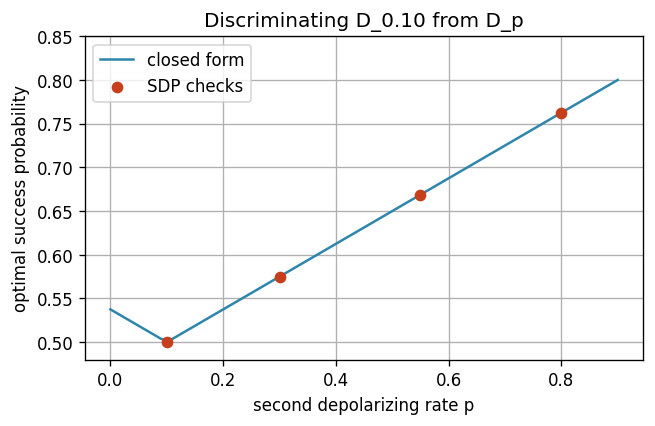
\includegraphics[width=0.72\textwidth]{fig_03_sdp_discrimination_01_cell9.png}
\caption{Depolarizing 매개변수 차이에 따른 구별 성공확률. 차이$\to0$이면 $p\to\tfrac12$, 차이가 커지면 정리 \ref{thm:chandisc}에 따라 $p$ 증가.}
\label{fig:sdp-depolarizing}
\end{figure}

\begin{figure}[H]
\centering
\begin{subfigure}{0.48\textwidth}\centering
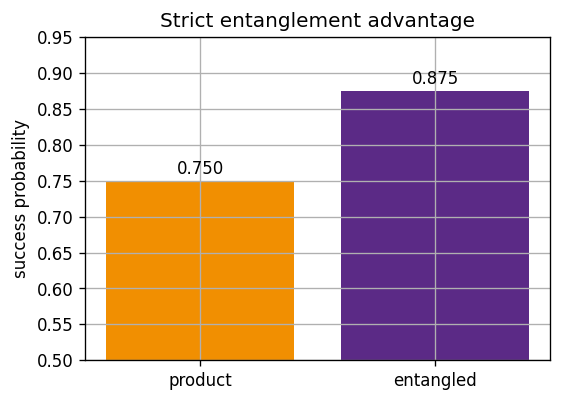
\includegraphics[width=\textwidth]{fig_03_sdp_discrimination_04_cell18.png}\caption{Product vs entangled}\end{subfigure}\hfill
\begin{subfigure}{0.48\textwidth}\centering
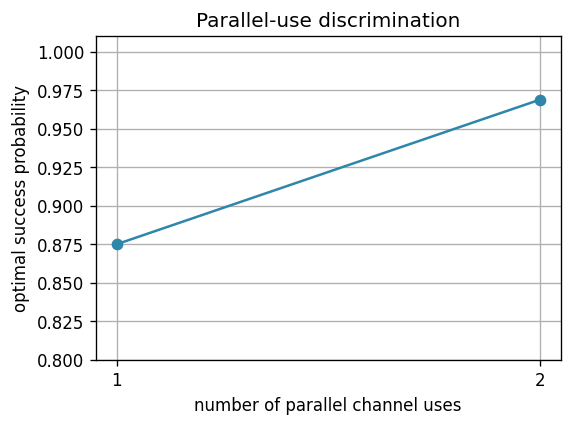
\includegraphics[width=\textwidth]{fig_03_sdp_discrimination_05_cell21.png}\caption{Parallel use}\end{subfigure}
\caption{얽힘과 반복 사용의 이점. product $0.750000$, ancilla-assisted $0.875000$, 2-shot parallel $0.968750$.}
\label{fig:sdp-advantage}
\end{figure}

\begin{property}[병렬 사용은 곱 채널의 diamond norm]
같은 채널을 $n$번 병렬 사용하는 전략의 성공확률은 $\tfrac12+\tfrac14\diamondnorm{\E_0^{\otimes n}-\E_1^{\otimes n}}$로, 차이가 누적되어 증가한다. 다만 $\Hcal_A^{\otimes n}$의 차원이 $d_A^n$으로 지수 증가하여 SDP 비용이 급증한다.
\end{property}

\begin{table}[H]
\centering
\begin{tabular}{lcc}
\toprule
전략 & 성공확률 & 근거 \\
\midrule
Bit-flip closed-form 검증 & 0.625000 & 해석적 $\diamondnorm{\cdot}$와 SDP(정리 \ref{thm:sdp}) 일치 → 구현 신뢰성. \\
Product input & 0.750000 & $\max_\rho\onenorm{\Delta(\rho)}$ (참조계 없음). \\
Ancilla-assisted input & 0.875000 & 전체 $\diamondnorm{\Delta}$ (정리 \ref{thm:chandisc}). \\
2-shot parallel & 0.968750 & $\diamondnorm{\Delta^{\otimes2}\text{형}}$, 차이 누적. \\
\bottomrule
\end{tabular}
\caption{SDP 기반 channel discrimination 결과}
\label{tab:sdp-results}
\end{table}

첫 줄(0.625)은 손으로 풀 수 있는 bit-flip 예의 \emph{해석적} diamond norm과 SDP 수치가 일치함을 보여, 정리 \ref{thm:sdp}의 구현이 옳음을 검증한다. 이후 $0.750\to0.875\to0.969$의 단조 증가는 각각 ``참조계 없음 $\to$ 참조계 얽힘 $\to$ 반복 사용''에 대응한다.

%==================================================================
\section{작업 4 --- Non-Markovian Dynamics와 Quantum Combs}
%==================================================================

\subsection{동역학 사상과 CP-divisibility}

\begin{definition}[동역학 사상과 분할가능성]
시간 매개변수화된 채널 족 $\{\Lambda(t)\}_{t\ge0}$($\Lambda(0)=\id$)을 동역학 사상(dynamical map)이라 한다. 두 시각 $t\ge s\ge0$에 대해 중간 전파자(propagator) $V(t,s)$를
\[
\Lambda(t)=V(t,s)\,\Lambda(s)
\]
로 정의한다($\Lambda(s)$가 가역일 때). 모든 $t\ge s$에서 $V(t,s)$가 CP이면 $\{\Lambda(t)\}$를 \textbf{CP-divisible}(Markovian의 한 정의)이라 한다.
\end{definition}

\begin{property}[CPTP의 trace-distance 수축성]\label{prop:contract}
임의의 CPTP 사상 $\Lambda$와 두 상태 $\rho,\sigma$에 대해
\[
T(\Lambda\rho,\Lambda\sigma)\le T(\rho,\sigma),\qquad T(\rho,\sigma)=\tfrac12\onenorm{\rho-\sigma}.
\]
즉 물리적(CP) 진화는 두 상태의 구별 가능성을 결코 증가시키지 못한다.
\end{property}

성질 \ref{prop:contract}이 핵심이다. \emph{trace distance가 증가하는 구간이 관측되면}, 그 구간의 중간 전파자 $V(t,s)$는 CP일 수 없다 --- 즉 CP-divisibility가 깨지고, 정보가 환경에서 계로 되돌아온 것이다.

\subsection{BLP measure: 정보 역류의 정량화}

\begin{definition}[BLP non-Markovianity measure]
$\sigma(t)=\dfrac{d}{dt}T\big(\Lambda(t)\rho_1,\Lambda(t)\rho_2\big)$라 할 때,
\[
\mathcal N_{\mathrm{BLP}}=\max_{\rho_1,\rho_2}\ \int_{\sigma(t)>0}\sigma(t)\,dt,
\]
즉 모든 초기 상태 쌍에 대해 trace distance가 \emph{증가}하는 구간만 합산한 양. $\mathcal N_{\mathrm{BLP}}>0$이면 non-Markovian.
\end{definition}

\begin{conceptbox}{개념: RHP-style witness}
RHP(Rivas--Huelga--Plenio) 관점은 중간 전파자 $V(t+\epsilon,t)$의 CP성을 직접 본다. $g(t)=\lim_{\epsilon\to0^+}\frac{1}{\epsilon}\big(\onenorm{(\id\otimes V(t+\epsilon,t))|\Omega\rangle\langle\Omega|}-1\big)$로 두면, $V$가 CP인 동안 $g(t)=0$이고, CP가 깨지면 $g(t)>0$. 이를 적분한 양이 RHP-style witness다. BLP가 ``정보 역류''를, RHP가 ``중간 단계의 비-CP성''을 본다.
\end{conceptbox}

\begin{figure}[H]
\centering
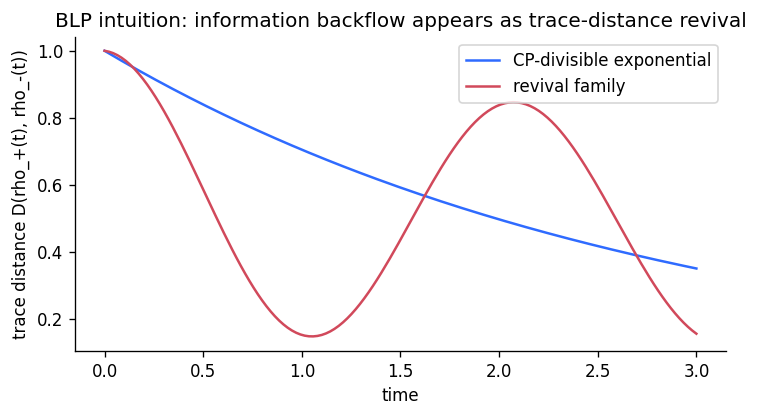
\includegraphics[width=0.76\textwidth]{fig_04_quantum_combs_01_cell7.png}
\caption{trace distance의 시간 변화. Markovian dephasing은 단조 감소($\sigma\le0$, 성질 \ref{prop:contract}와 부합), revival dephasing은 재증가 구간($\sigma>0$) 존재 → $\mathcal N_{\mathrm{BLP}}>0$.}
\label{fig:comb-trace-distance}
\end{figure}

\subsection{Quantum comb와 link product}

\begin{definition}[quantum comb]
다중 시점 과정을 $\Hcal_0\otimes\Hcal_1\otimes\cdots\otimes\Hcal_{2N-1}$(번갈아 input/output) 위 PSD 연산자 $C\succeq0$로 나타낸 것을 $N$-comb이라 한다. 인과(causality) 구조는 부분 대각합 조건의 위계로 표현된다. 예컨대 2-comb($\Hcal_0\,\text{in},\Hcal_1\,\text{out},\Hcal_2\,\text{in},\Hcal_3\,\text{out}$)는
\[
\Tr_{3}\,C=I_{2}\otimes C^{(1)},\qquad \Tr_{1}\,C^{(1)}=I_{0},
\]
를 만족해야 한다(Chiribella--D'Ariano--Perinotti). 이는 정리 \ref{thm:cj}의 TP 조건($\Tr_B C_\E=I_A$)을 여러 시점으로 확장한 것이다.
\end{definition}

\begin{definition}[link product과 memoryless product]
두 comb의 합성은 공유 계에 대한 부분 대각합과 전치를 결합한 \textbf{link product} $\star$로 주어진다. 시점 사이에 상관이 전혀 없는 ``기억 없는'' 과정은 각 시점 marginal $C^{(k)}$의 텐서곱
\[
C_{\mathrm{prod}}=\bigotimes_k C^{(k)}
\]
으로 분해된다. \textbf{상대 상관 노름}
\[
\eta=\frac{\onenorm{C-C_{\mathrm{prod}}}}{\onenorm{C}}
\]
이 0이 아니면 시점 간 상관(기억)이 존재한다.
\end{definition}

\begin{figure}[H]
\centering
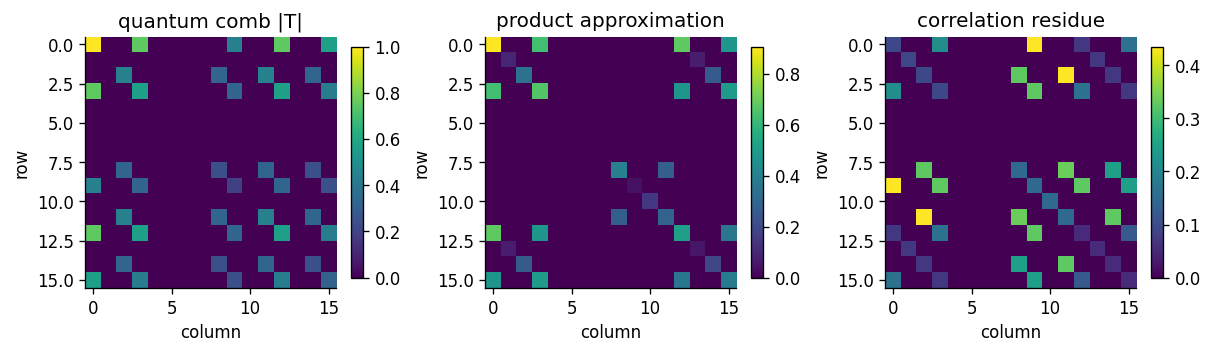
\includegraphics[width=0.92\textwidth]{fig_04_quantum_combs_02_cell10.png}
\caption{Two-use collision model의 comb, memoryless product, 그리고 차이. 차이$\neq0\Rightarrow$ 시점 간 상관 존재.}
\label{fig:comb-correlation}
\end{figure}

\begin{mathbox}{collision model의 수치 검증}
구성된 comb는 $C\in\Lin(\mathbb C^{16})$, 최소 고유값 $-1.774\times10^{-16}=\mathcal O(\varepsilon_{\mathrm{mach}})\Rightarrow C\succeq0$(물리적). 인과 위계(causality hierarchy)=True. 그러나 곱 분해 가능성(product marginal factorization)=False이고
\[
\eta=\frac{\onenorm{C-C_{\mathrm{prod}}}}{\onenorm{C}}\approx0.5307\neq0.
\]
\textbf{이 $\eta\neq0$이 기억 효과의 정량적 핵심 증거다.}
\end{mathbox}

\begin{figure}[H]
\centering
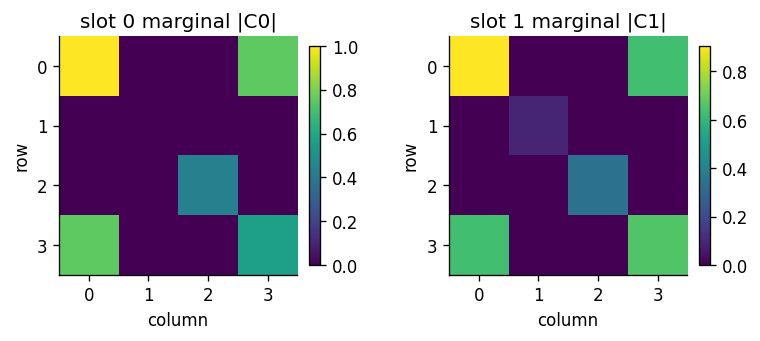
\includegraphics[width=0.72\textwidth]{fig_04_quantum_combs_03_cell13.png}
\caption{각 slot의 marginal Choi. 개별로는 정상적 1단계 채널이나, 곱만으로 전체 comb를 복원 불가($\eta\neq0$). 기억은 ``개별 시점''이 아니라 ``시점 간 상관''에 있다.}
\label{fig:comb-marginals}
\end{figure}

\begin{table}[H]
\centering
\begin{tabular}{lcc}
\toprule
Channel family & BLP grid estimate & RHP-style grid witness \\
\midrule
Exponential dephasing & 0.000000 & 0.000000 \\
Revival dephasing & 0.699240 & 0.896321 \\
\bottomrule
\end{tabular}
\caption{비마르코프성 witness 결과. 두 독립 진단(정보 역류 / 중간 단계 비-CP)이 같은 결론.}
\label{tab:nonmarkov-results}
\end{table}

exponential dephasing은 $\mathcal N_{\mathrm{BLP}}=0$이고 RHP$=0$(CP-divisible). revival dephasing은 둘 다 양수로, 정의가 다른 두 measure가 동일하게 non-Markovian을 가리킨다 --- 결과의 robust함을 보여준다.

%==================================================================
\section{작업 5 --- Interactive Widget: 조건의 시각적 동치}
%==================================================================

Widget은 정리 \ref{thm:cj}의 두 조건을 \emph{실시간으로} 보여준다. 매개변수를 바꿀 때 다음이 동시에 갱신된다.
\[
\underbrace{\text{Choi eigenspectrum}}_{C_\E\succeq0?\ (\text{CP})},\quad
\underbrace{\Tr_B(C_\E)}_{=I_A?\ (\text{TP})},\quad
\underbrace{\text{Kraus }\{K_k\}}_{\text{정리 \ref{thm:cj}}},\quad
\underbrace{\vec r\mapsto M\vec r+\vec t}_{\text{Bloch}}.
\]

\begin{figure}[H]
\centering
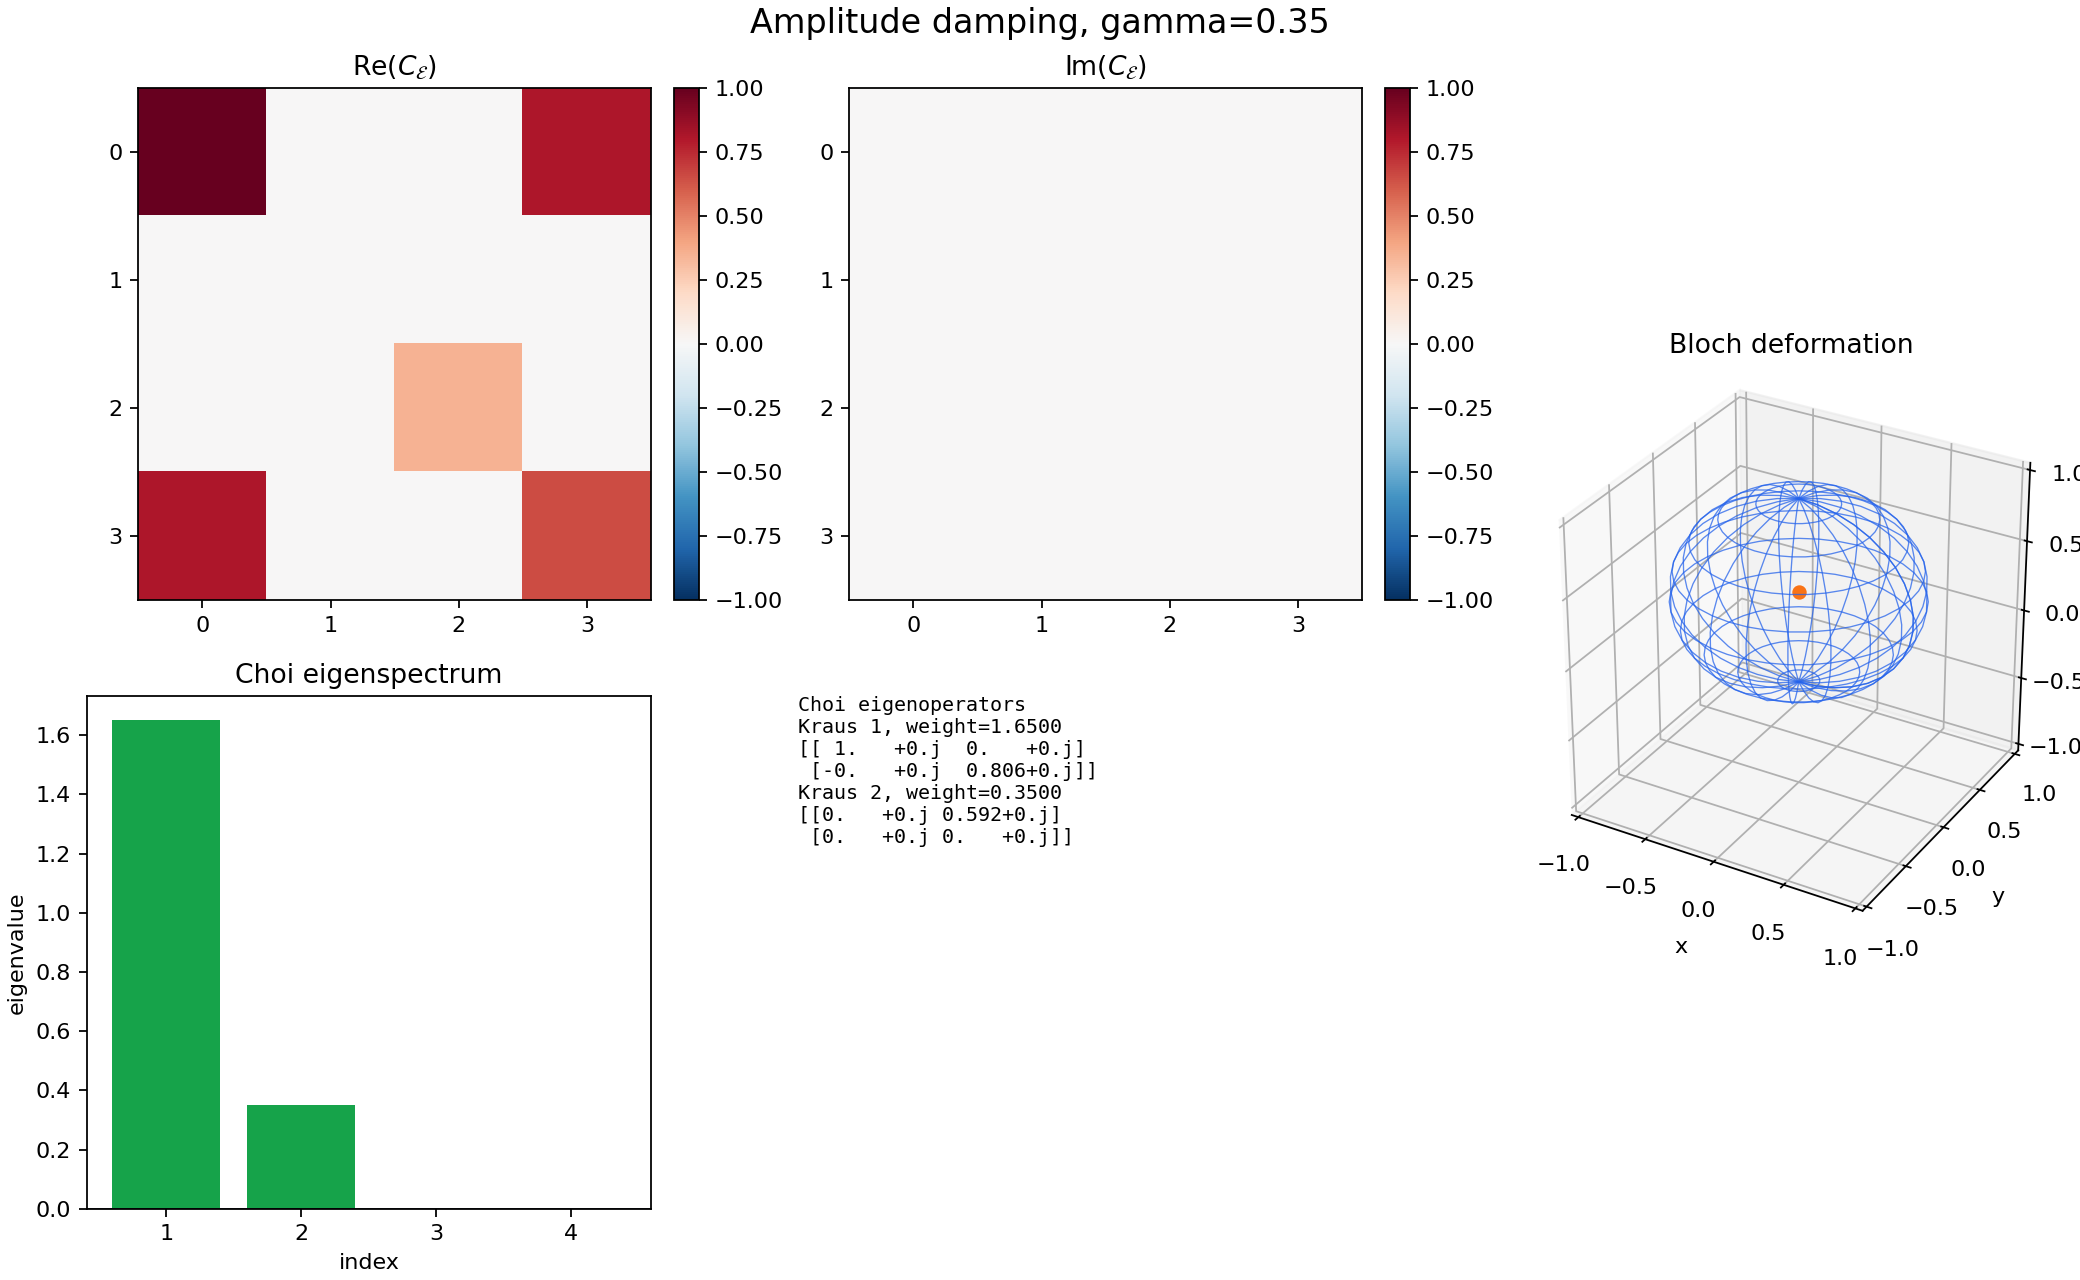
\includegraphics[width=0.94\textwidth]{fig_widget_dashboard.png}
\caption{amplitude damping 예시. Choi 실수부/허수부/절댓값(좌), Choi 고유값과 Bloch 변형(우). $\vec t=(0,0,\gamma)\neq0$이므로 구의 중심이 이동 --- 비-unital성의 시각적 표현(4.1절 amplitude damping 상자).}
\label{fig:widget-dashboard}
\end{figure}

\begin{property}[CP 경계의 시각적 신호]
사용자가 매개변수를 CP 영역 밖으로 옮기면 $C_\E$에 음의 고유값이 나타난다(정리 \ref{thm:cj} 위반). 행렬 성분의 변화는 작아 보여도 $\min\mathrm{eig}(C_\E)<0$이 되는 순간 채널은 비물리적이다 --- 4.3절 perturbed identity, 5.4절 비물리적 재구성과 같은 현상의 대화형 버전.
\end{property}

따라서 widget은 작업 1의 CP/TP 판정, 작업 2의 잡음 진단($M,\vec t$), 작업 3의 채널 차이를 한 화면에서 잇는다.

%==================================================================
\section{통합 해석: 하나의 좌표계로서의 Choi 행렬}
%==================================================================

\begin{longtable}{p{0.16\textwidth}p{0.40\textwidth}p{0.32\textwidth}}
\toprule
파트 & Choi 행렬의 수학적 역할 & 핵심 식 \\
\midrule
이론 & 표현 변환·물리성 판정 & $C_\E\succeq0$(CP), $\Tr_B C_\E=I_A$(TP) \\
Tomography & 재구성 대상 & $\E(\rho)=\Tr_A[(\rho^T\otimes I)C_\E]$, $F_{\mathrm{avg}}=\frac{dF_{\mathrm{pro}}+1}{d+1}$ \\
SDP & 최적화 입력 데이터 & $p=\tfrac12+\tfrac14\diamondnorm{\E_0-\E_1}$ \\
Combs & 다중 시점으로 확장 & $\Tr_3 C=I_2\otimes C^{(1)}$, $\eta=\onenorm{C-C_{\mathrm{prod}}}/\onenorm{C}$ \\
Widget & 조건의 동치 표현 & $\min\mathrm{eig}(C_\E)\gtrless0$ \\
\bottomrule
\caption{Choi 표현의 통합적 역할(수식 요약)}
\label{tab:integration}
\end{longtable}

종합하면, Choi 행렬은 단일 선형 대상 $C_\E\in\Lin(\Hcal_A\otimes\Hcal_B)$ 위에서 (i)~물리성을 \emph{판정}하고($\succeq0$, $\Tr_B=I$), (ii)~재구성의 \emph{대상}이 되며, (iii)~두 행렬의 차이가 최적화의 \emph{입력}이 되고($\diamondnorm{\cdot}$), (iv)~다중 시점으로 \emph{확장}된다(comb). 같은 표현을 끝까지 유지했기에 다섯 작업의 결과가 하나의 식 체계로 연결된다.

\paragraph{한계(수식적 관점).}
$C_\E\in\Lin(\Hcal_A\otimes\Hcal_B)$의 크기는 $d_Ad_B$이고 SDP 변수는 $\mathcal O((d_Ad_B)^2)$. $N$-comb은 $\prod_k d_k$로 차원이 \emph{지수} 증가($\eta$ 계산 비용도 함께). 따라서 대규모로 가려면 대칭성, tensor network, randomized benchmarking 같은 압축이 필요하다. 또한 tomography 수치는 offline simulated fixture 기반이므로, 표의 $F_{\mathrm{pro}}$/diamond 값을 실제 하드웨어 성능으로 해석해서는 안 된다.

%==================================================================
\section{결론}
%==================================================================

이 해설본은 ``Choi 행렬을 쓰면 채널 분석이 선형대수로 환원된다''는 주장을 정의·성질·정리로 재구성했다. 핵심은 \textbf{Choi--Jamio{\l}kowski 동형사상}(정리 \ref{thm:cj})으로,
\[
\E\text{ CP}\iff C_\E\succeq0,\qquad \E\text{ TP}\iff\Tr_B(C_\E)=I_A
\]
이라는 두 등가성이 이후 모든 작업의 토대가 되었다. 그 위에서 표현 변환의 일관성($\mathcal O(\varepsilon_{\mathrm{mach}})$ 오차), fidelity 관계식($F_{\mathrm{avg}}=\frac{dF_{\mathrm{pro}}+1}{d+1}$로 표 재현), 채널 구별의 operational 의미($p=\tfrac12+\tfrac14\diamondnorm{\cdot}$와 Watrous SDP), 정보 역류의 정량화(trace-distance 수축성과 BLP/RHP), 다중 시점 상관($\eta=\onenorm{C-C_{\mathrm{prod}}}/\onenorm{C}$)을 모두 수식으로 제시했다. 같은 행렬 $C_\E$가 물리성 판정자, 재구성 대상, 최적화 데이터, 시간 확장 객체로 동시에 작동한다는 점이 이 프로젝트의 통합적 결론이다.

\section*{참고문헌}
\addcontentsline{toc}{section}{참고문헌}
\begin{itemize}
  \item M. A. Nielsen and I. L. Chuang, \textit{Quantum Computation and Quantum Information}. Cambridge University Press, 2010.
  \item M.-D. Choi, ``Completely positive linear maps on complex matrices,'' \textit{Linear Algebra and its Applications}, 1975.
  \item A. Jamio{\l}kowski, ``Linear transformations which preserve trace and positive semidefiniteness of operators,'' \textit{Reports on Mathematical Physics}, 1972.
  \item J. Watrous, \textit{The Theory of Quantum Information}. Cambridge University Press, 2018.
  \item J. Watrous, ``Semidefinite programs for completely bounded norms,'' \textit{Theory of Computing}, 2009.
  \item M. Horodecki, P. Horodecki, and R. Horodecki, ``General teleportation channel, singlet fraction, and quasidistillation,'' \textit{Physical Review A}, 1999. (process/average fidelity 관계)
  \item G. Chiribella, G. M. D'Ariano, and P. Perinotti, ``Quantum circuit architecture,'' \textit{Physical Review Letters}, 2008.
  \item H.-P. Breuer, E.-M. Laine, and J. Piilo, ``Measure for the degree of non-Markovian behavior of quantum processes,'' \textit{Physical Review Letters}, 2009.
  \item Á. Rivas, S. F. Huelga, and M. B. Plenio, ``Entanglement and non-Markovianity of quantum evolutions,'' \textit{Physical Review Letters}, 2010.
\end{itemize}

\end{document}
